\section{Manuel d’utilisateur}

\begin{wrapfigure}{r}{0.3\linewidth}
    \centering
    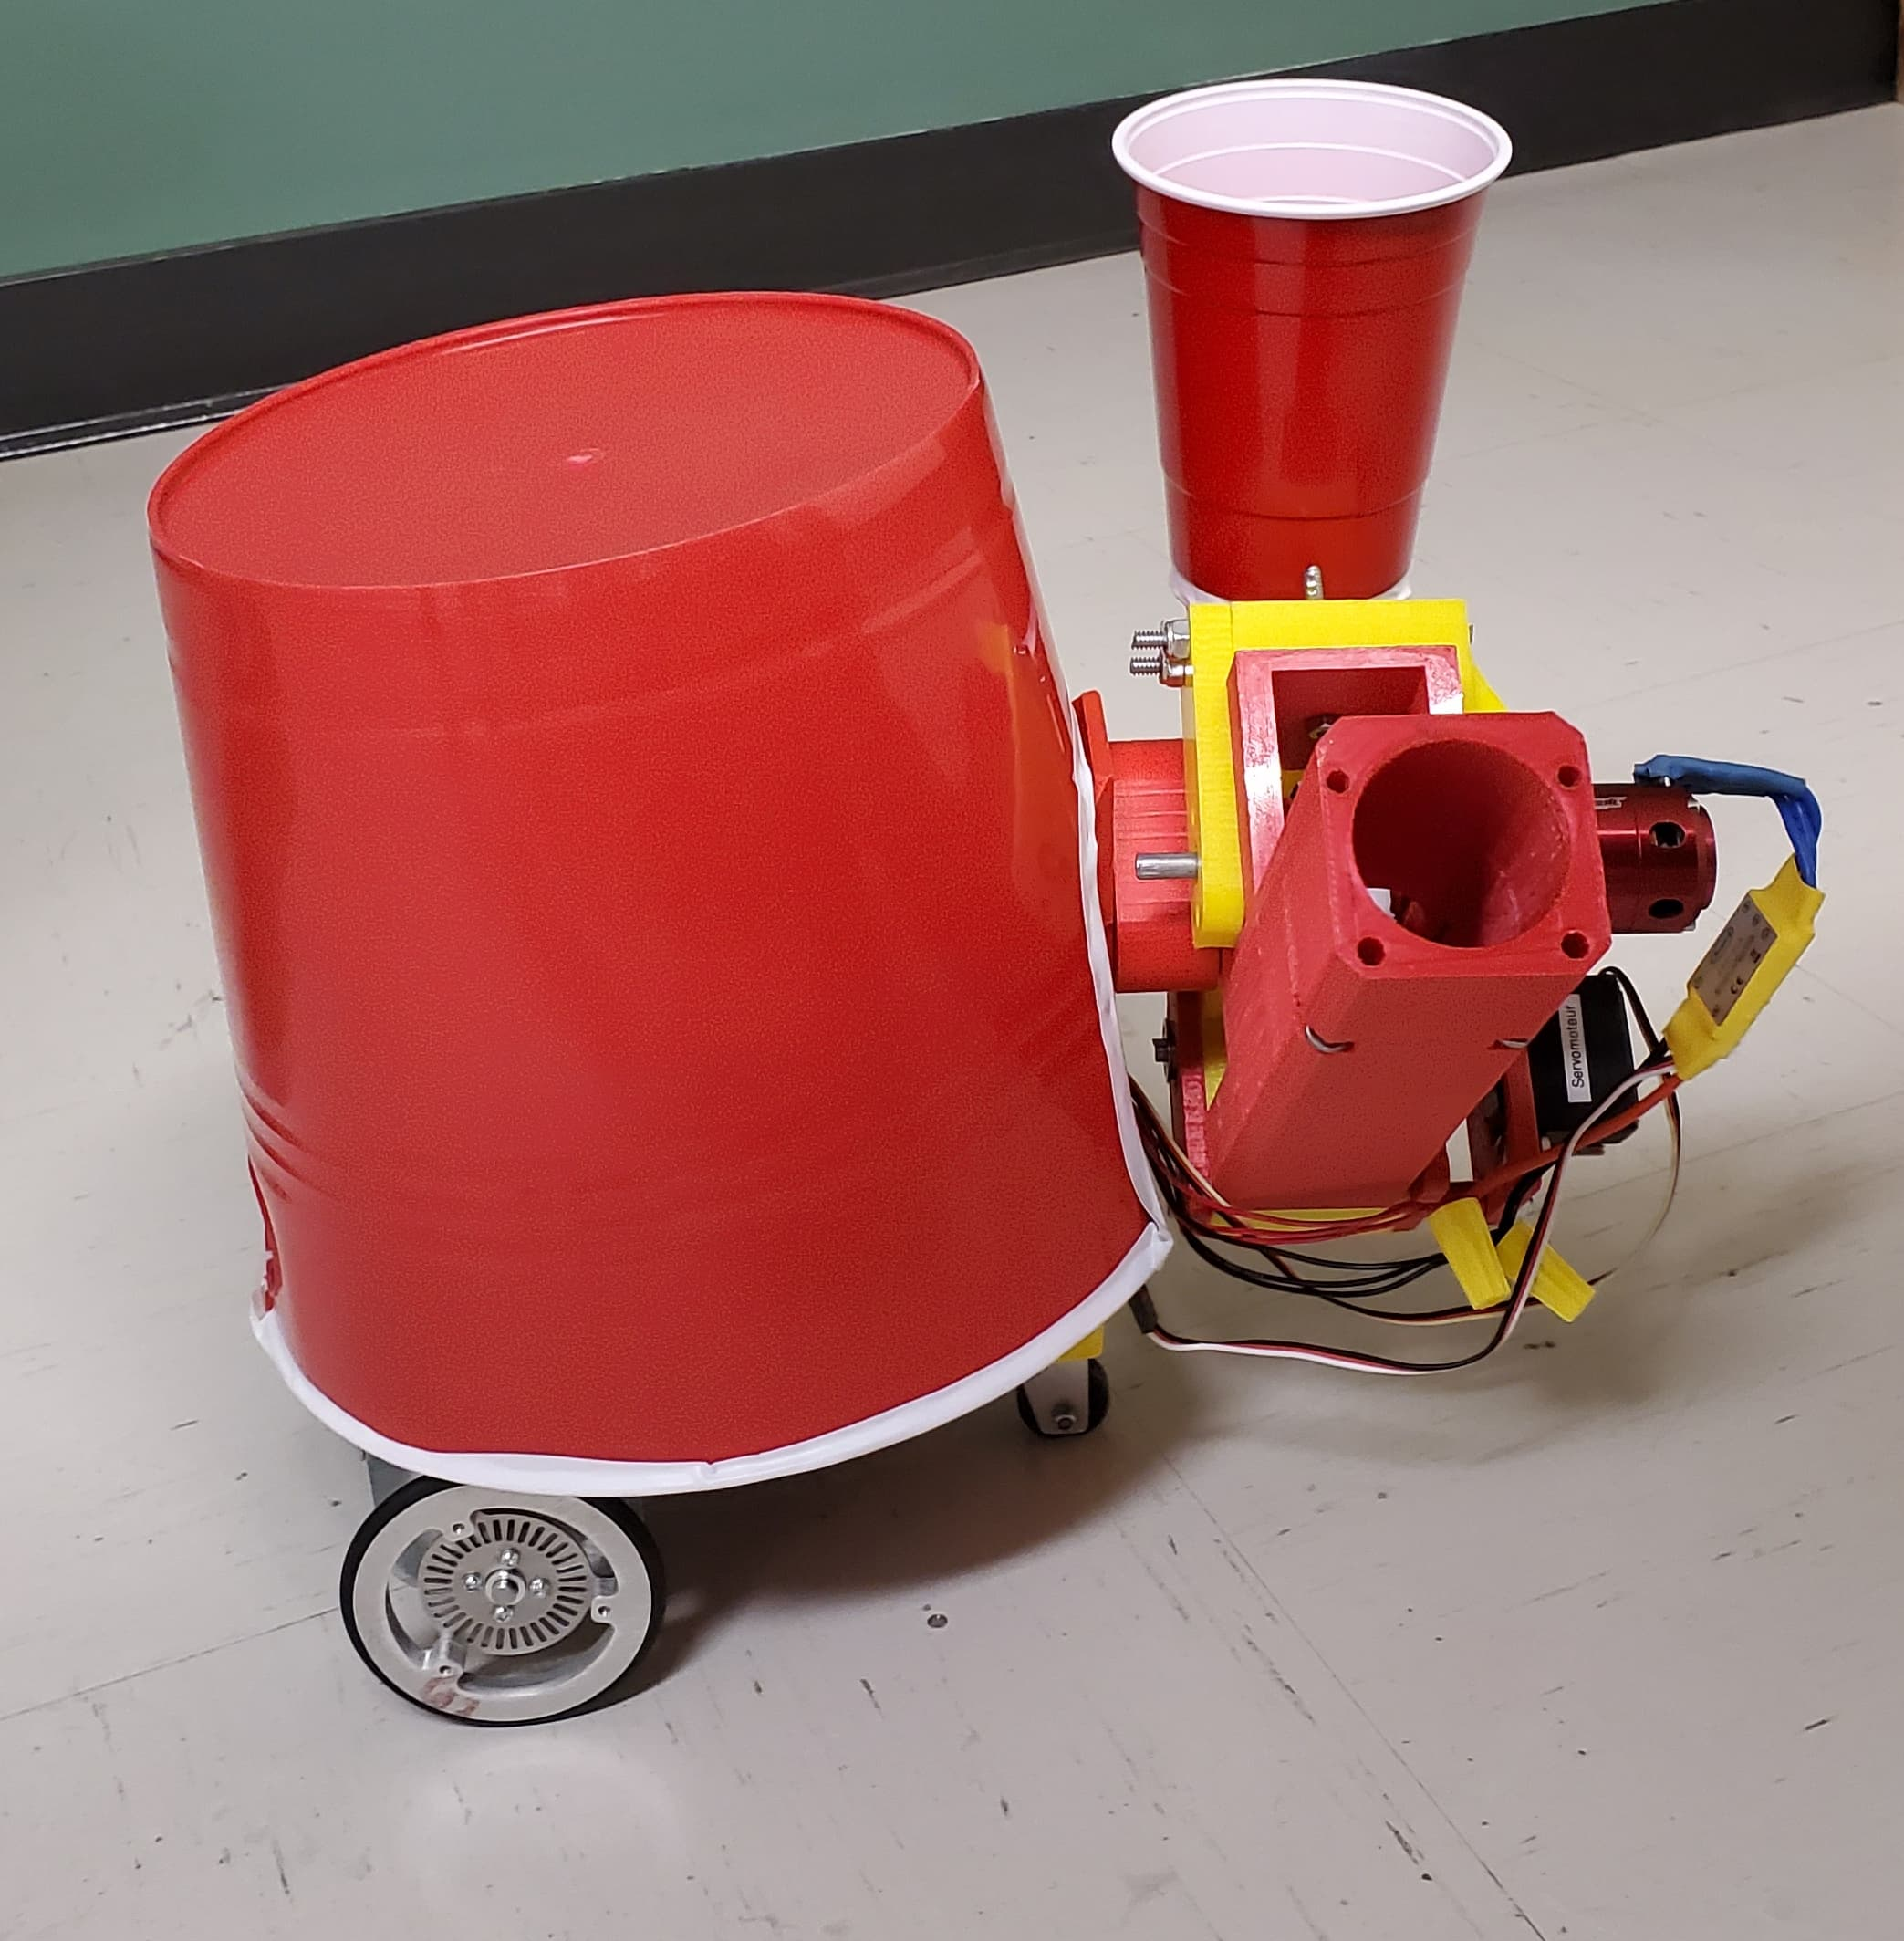
\includegraphics[width=\linewidth]{img/a1/protoype}
    \caption{Version finale du prototype}
    \label{fig:a1-protoype}
\end{wrapfigure}

Le robot est un lanceur de balle de bière-pong qui a comme utilisation première de lancer des balles dans des verres.
Le robot sera contrôlé par un utilisateur à l’aide d’une application mobile qui lui permettra de le faire bouger de gauche à droite et de contrôler la force du moteur avec de lancer la balle.
De plus, des verres intelligents accompagnent le robot.
Les verres détectent les balles à l’intérieur du verre pour avertir le joueur quels verres sont réussis à l’aide de lumières qui s’allument.

\subsection{Installation de l’application}

\begin{enumerate}
    \item Créer un compte \href{https://appinventor.mit.edu/}{MIT App Inventor (https://appinventor.mit.edu/)}.
    \item Obtenir l’application sur son compte MIT App Inventor.
    \item Construire le code QR de l’application à l’aide d’un outil de MIT App Inventor (figure~\ref{fig:a1-create-code-QR})
    \item Avec un téléphone Android, numériser le code QR, afin que l’application s’installe sur votre téléphone. (figure~\ref{fig:a1-code-QR})
    \item Vous pouvez maintenant lancer l’application à l’aide de l’icône qui s’est installer sur votre téléphone. (figure~\ref{fig:a1-app-icon})
\end{enumerate}

\begin{figure}[h!]
    \centering

    \begin{subfigure}{0.5\linewidth}
        \centering
        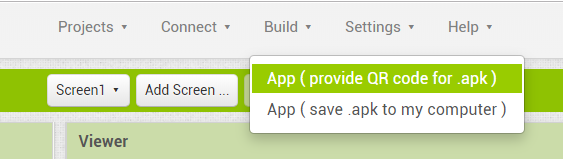
\includegraphics[width=\linewidth]{img/a1/create-code-QR}
        \caption{Construction du code QR}
        \label{fig:a1-create-code-QR}
    \end{subfigure}
    \begin{subfigure}{0.2\linewidth}
        \centering
        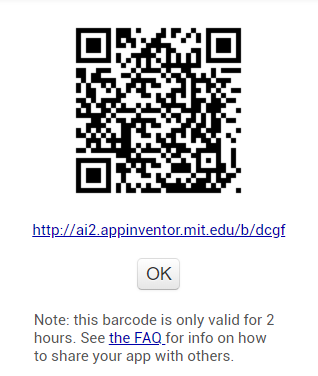
\includegraphics[width=\linewidth]{img/a1/code-QR}
        \caption{Code QR}
        \label{fig:a1-code-QR}
    \end{subfigure}
    \begin{subfigure}{0.2\linewidth}
        \centering
        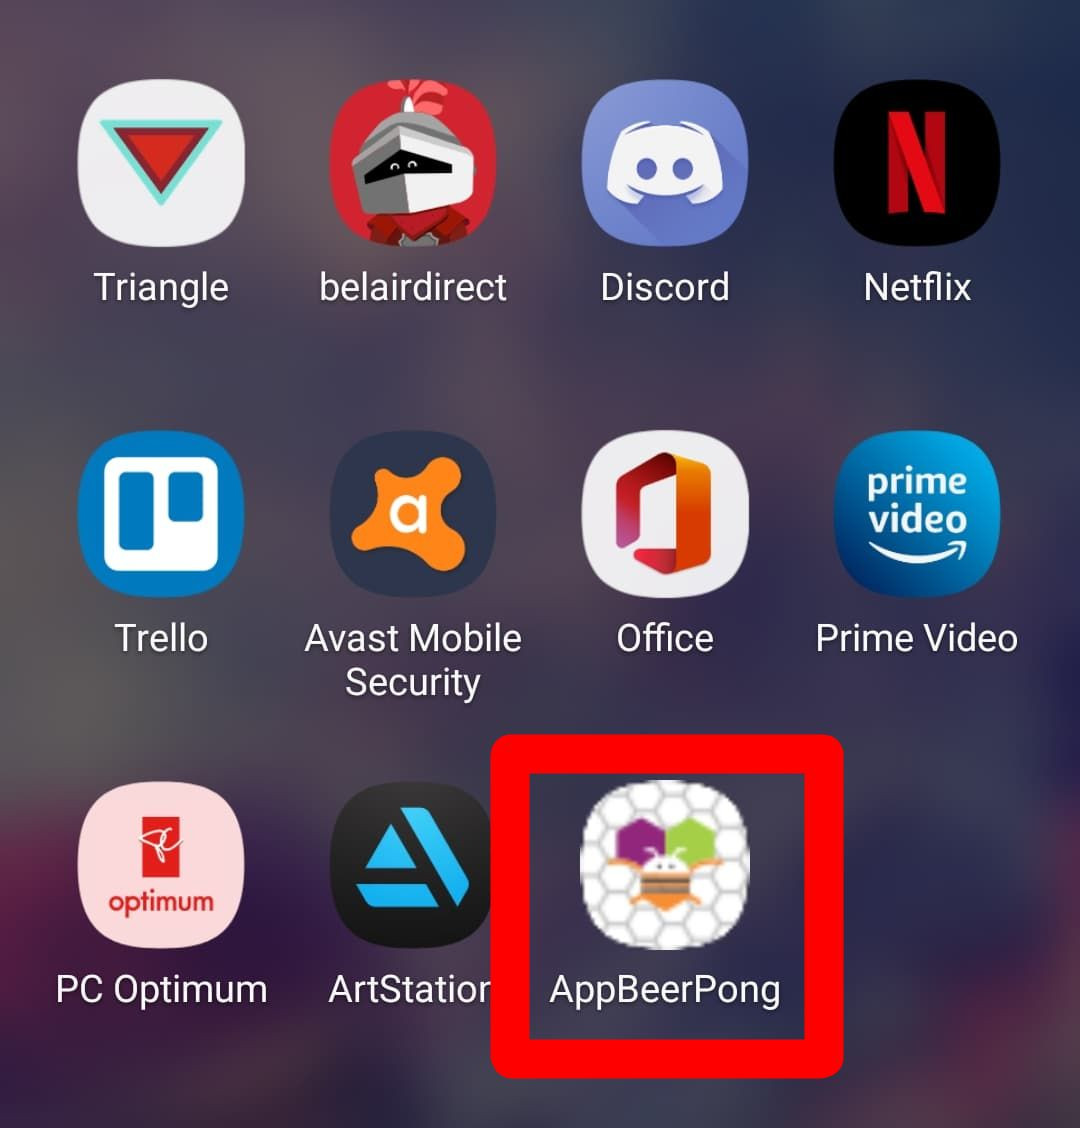
\includegraphics[width=\linewidth]{img/a1/app-icon}
        \caption{Icône de l’application}
        \label{fig:a1-app-icon}
    \end{subfigure}

    \caption{Installation de l’application}
    \label{fig:a1-install-app}
\end{figure}

\subsection{Mise en marche du robot}

\begin{enumerate}
    \item Soulever le chapeau du robot. 
    \item Pour mettre en marche le robot il faut activer l’interrupteur. (figure~\ref{fig:a1-interrupteur})
    \item Si le robot manque de puissance il faut penser à recharger la batterie qui se situe sous le robot. (figure~\ref{fig:a1-chargeur-batterie})
    \item Remplir le réservoir du robot, afin de pouvoir lancer des balles.
    \item Placer le robot en face des verres à une distance raisonnable.
\end{enumerate}

\subsection{Mise en marche du plateau des verres}

\begin{enumerate}
    \item Il suffit d’activer les deux interrupteurs sur la boite noire de la plateforme des verres. (figure~\ref{fig:a1-interrupteur-verres})
    \item Si les lumières n’allument pas, il faut changer les batteries (2 batteries 9~V) dans la boite noire collée au module des verres.
\end{enumerate}

\begin{figure}[h!]
    \centering

    \begin{subfigure}{0.3\linewidth}
        \centering
        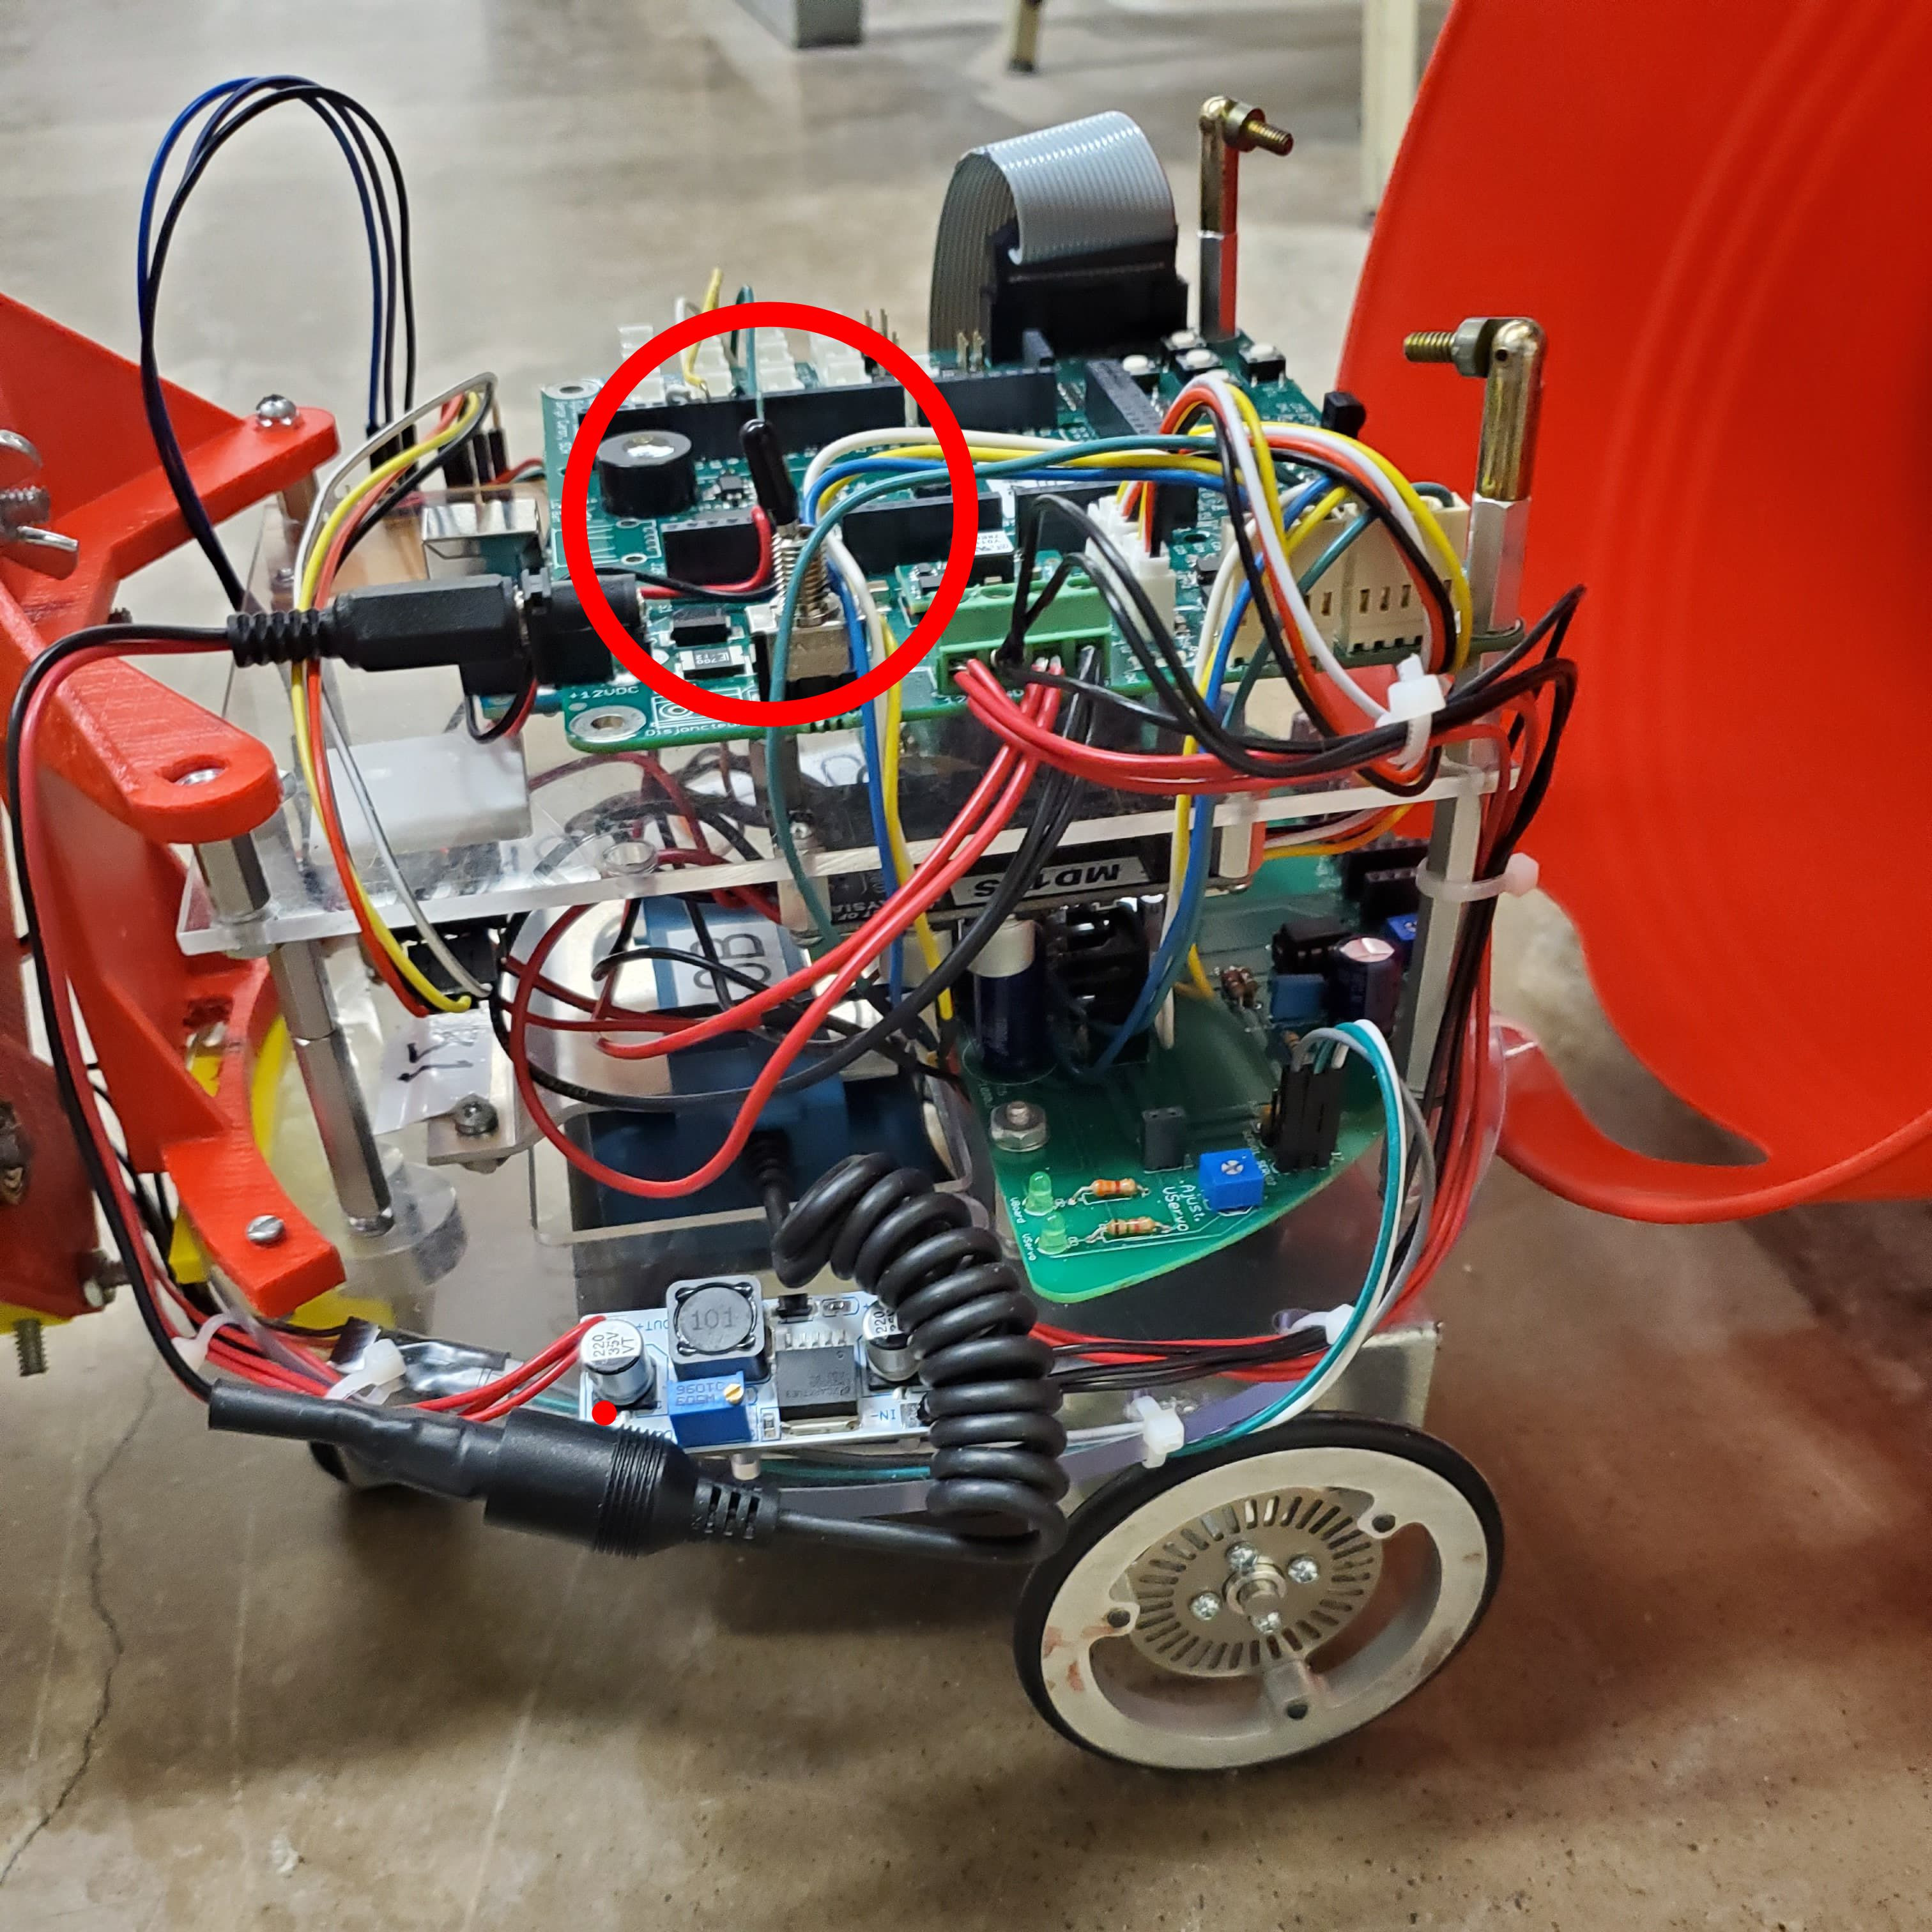
\includegraphics[width=\linewidth]{img/a1/interrupteur}
        \caption{Interrupteur du robot}
        \label{fig:a1-interrupteur}
    \end{subfigure}
    \begin{subfigure}{0.3\linewidth}
        \centering
        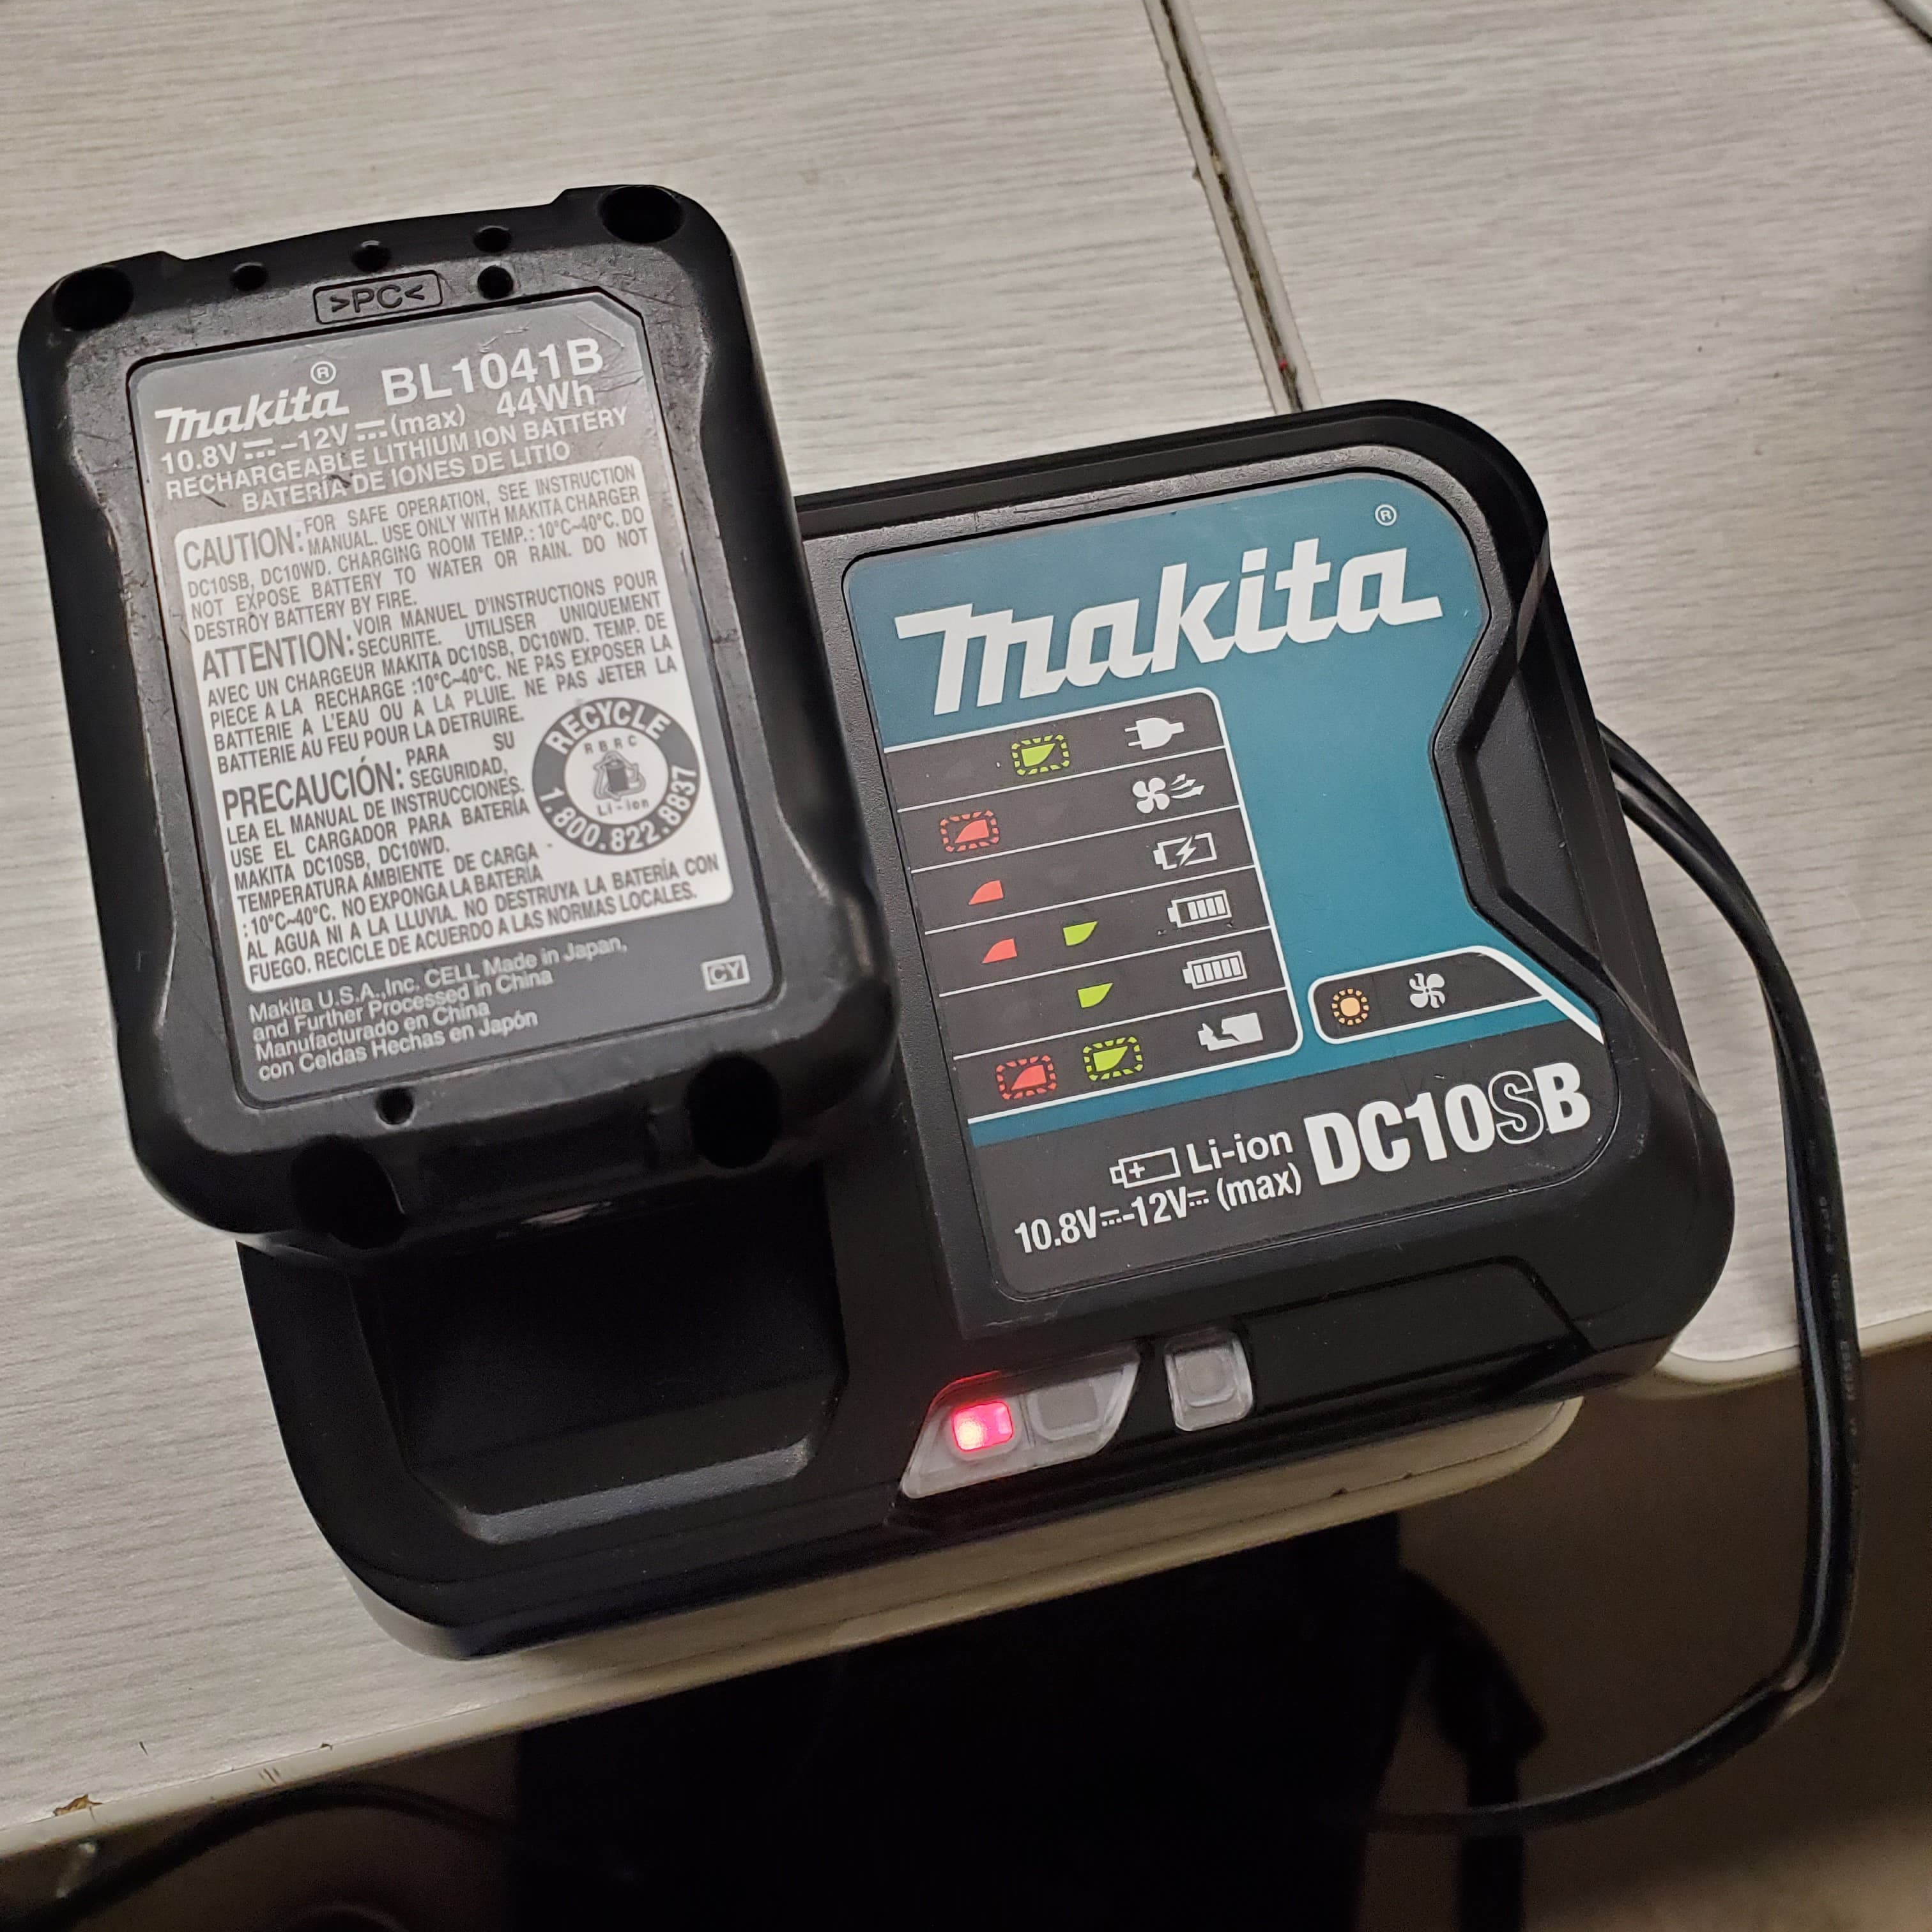
\includegraphics[width=\linewidth]{img/a1/chargeur-batterie}
        \caption{Chargeur de batterie}
        \label{fig:a1-chargeur-batterie}
    \end{subfigure}
    \begin{subfigure}{0.3\linewidth}
        \centering
        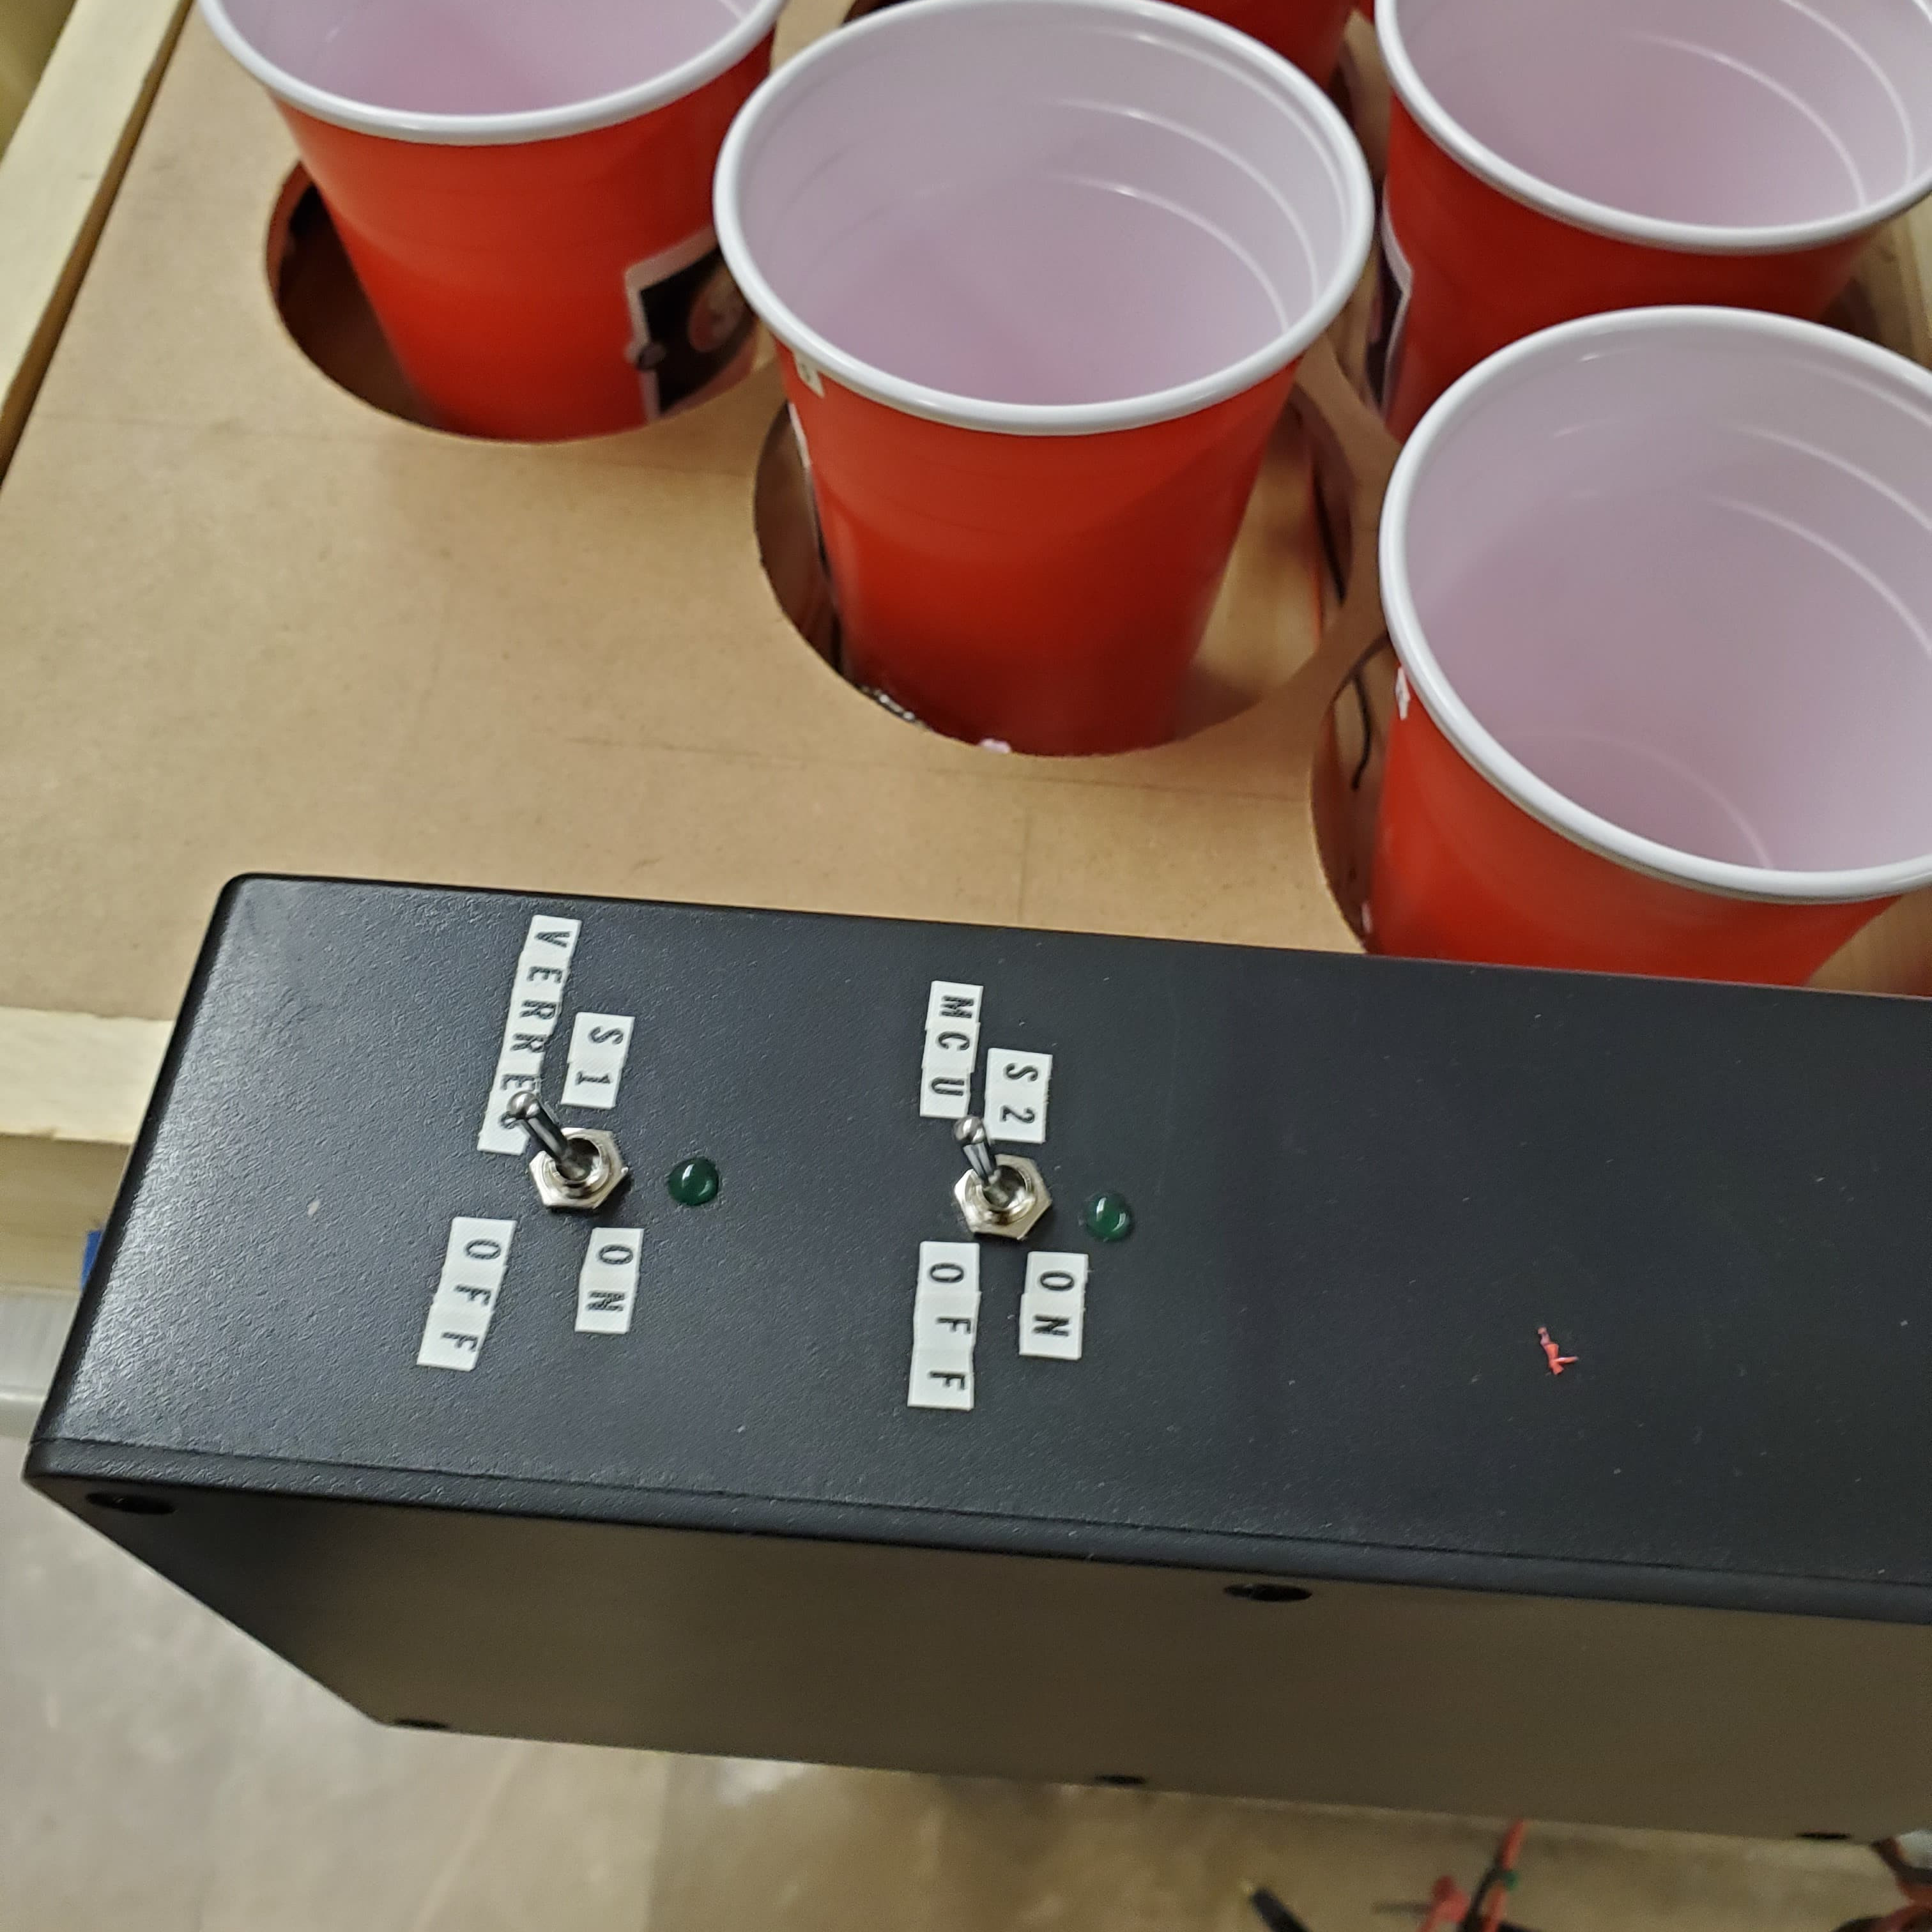
\includegraphics[width=\linewidth]{img/a1/interrupteur-verres}
        \caption{Interrupteur du plateau}
        \label{fig:a1-interrupteur-verres}
    \end{subfigure}

    \caption{Mise en marche du robot et du plateau de verres}
    \label{fig:a1-demarrage-robot}
\end{figure}

\subsection{Connection de l'application au robot}

\begin{enumerate}
    \item Aller dans vos réglages Bluetooth de votre téléphone pour vous connecter au périphérique \texttt{HC05-Slave}
    \item Rentrer le mot de passe: 1234
    \item Aller dans l’application et utiliser le bouton Bluetooth pour se connecter au Bluetooth du robot. (bouton 7 dans la figure~\ref{fig:a1-Application})
    \item Sélectionner \texttt{00.18:E4:34:DC:A0 HC05-Slave} (figure~\ref{fig:a1-app-Bluethooth})
    \item Quand le robot a été arrêté vous devez refaire les étapes 3 et 4
\end{enumerate}

\subsection{Contrôle du robot avec l’application}

\begin{enumerate}
    \item Pour faire bouger le robot à gauche utiliser le bouton en haut à gauche de l’application (bouton 1 dans la figure~\ref{fig:a1-Application})
    \item Pour faire bouger le robot à droite utiliser le bouton en haut à droite de l’application (bouton 2 dans la figure~\ref{fig:a1-Application})
    \item Pour faire augmenter la puissance du moteur utiliser le bouton d’addition (bouton 3 dans la figure~\ref{fig:a1-Application})
    \item Pour diminuer la puissance du moteur utiliser le bouton de soustraction (bouton 4 dans la figure~\ref{fig:a1-Application})
    \item Pour lancer la balle utiliser le bouton en forme de balle de ping-pong (bouton 6 dans la figure~\ref{fig:a1-Application})
\end{enumerate}


\begin{figure}[h!]
    \centering
    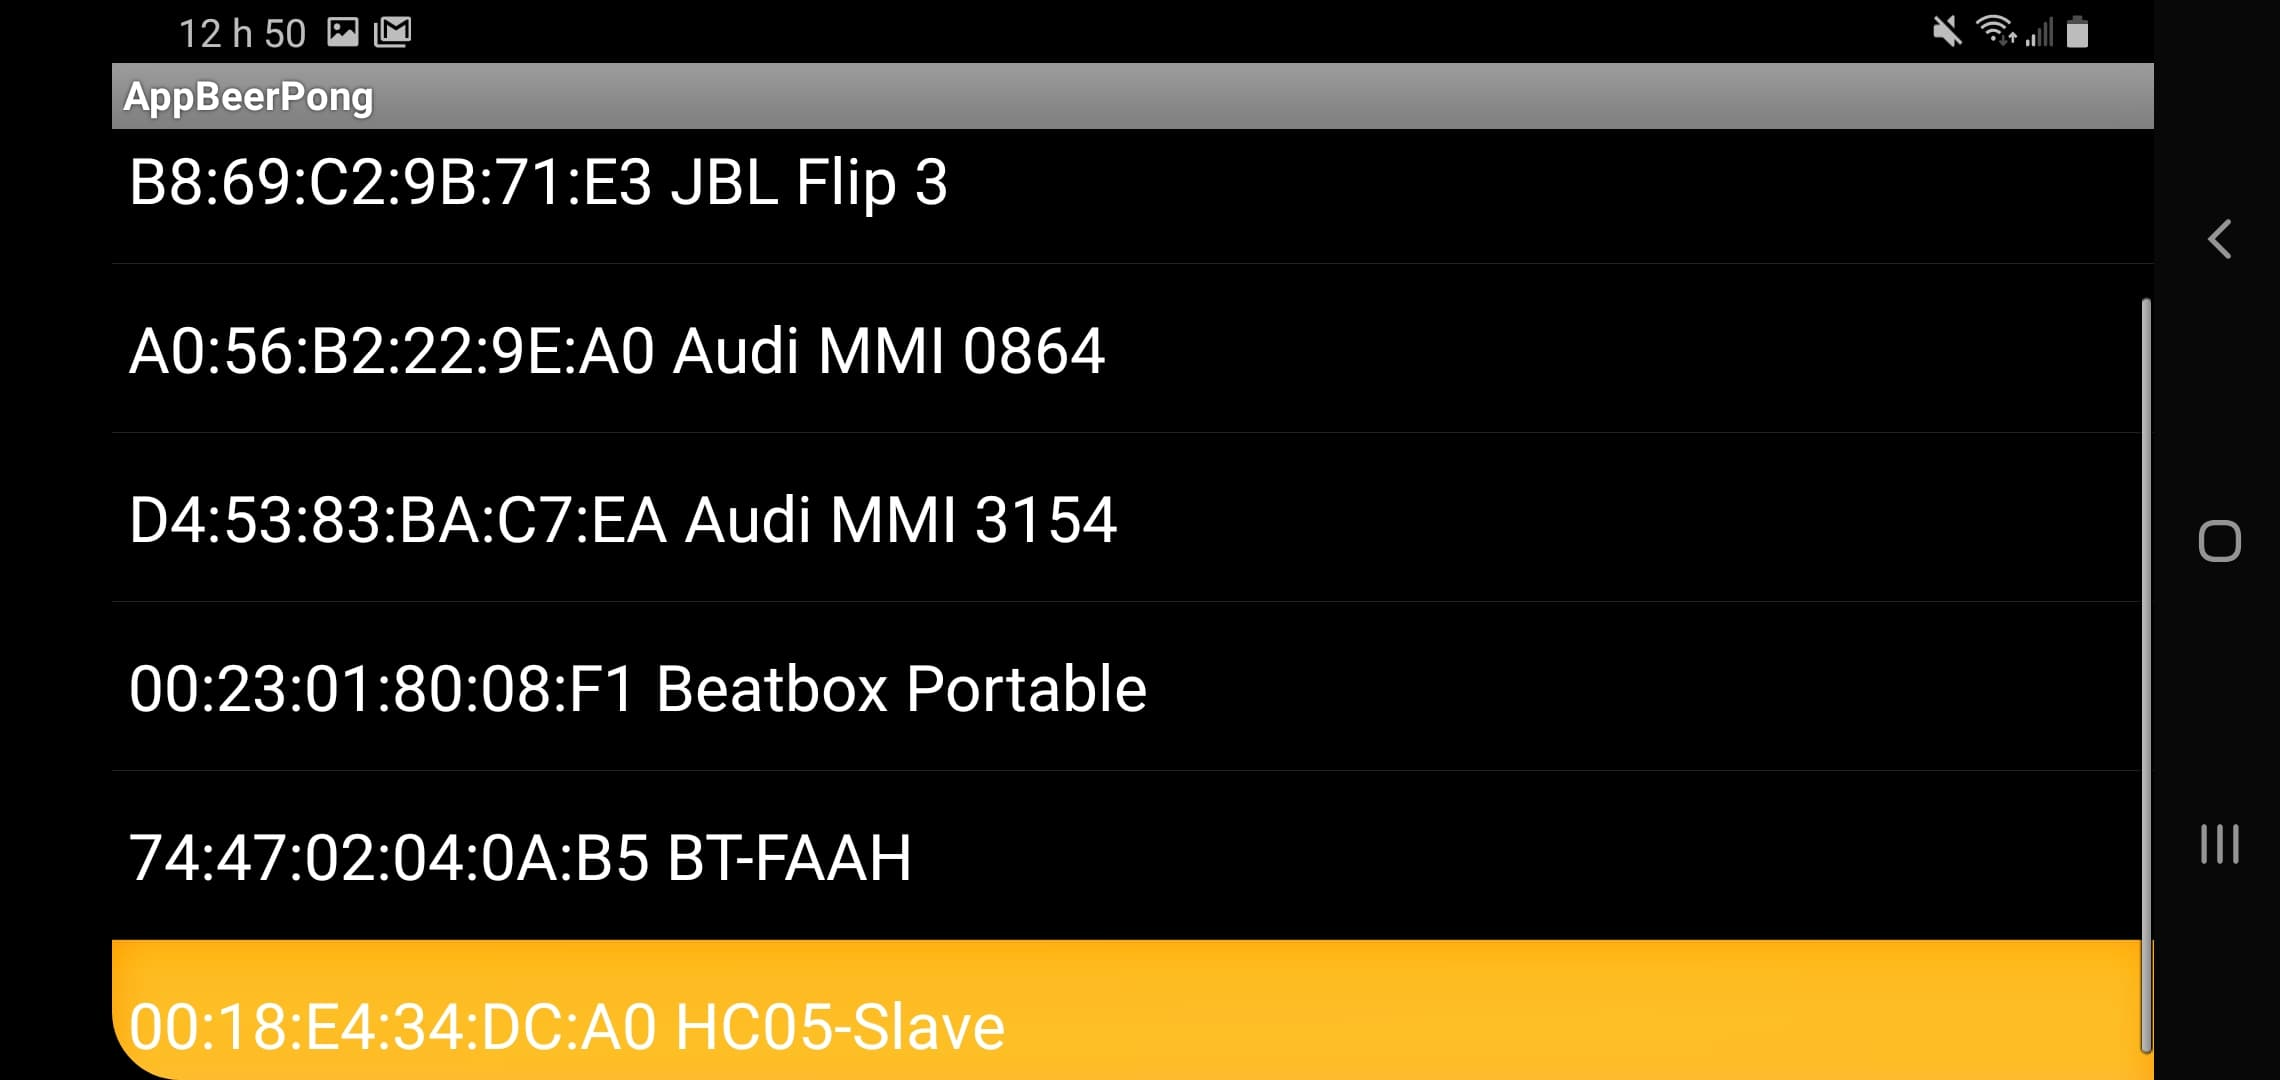
\includegraphics[width=0.6\linewidth]{img/a1/app-Bluethooth}
    \caption{Paramètres Bluetooth de l'application}
    \label{fig:a1-app-Bluethooth}
\end{figure}

\begin{figure}[h!]
    \centering
    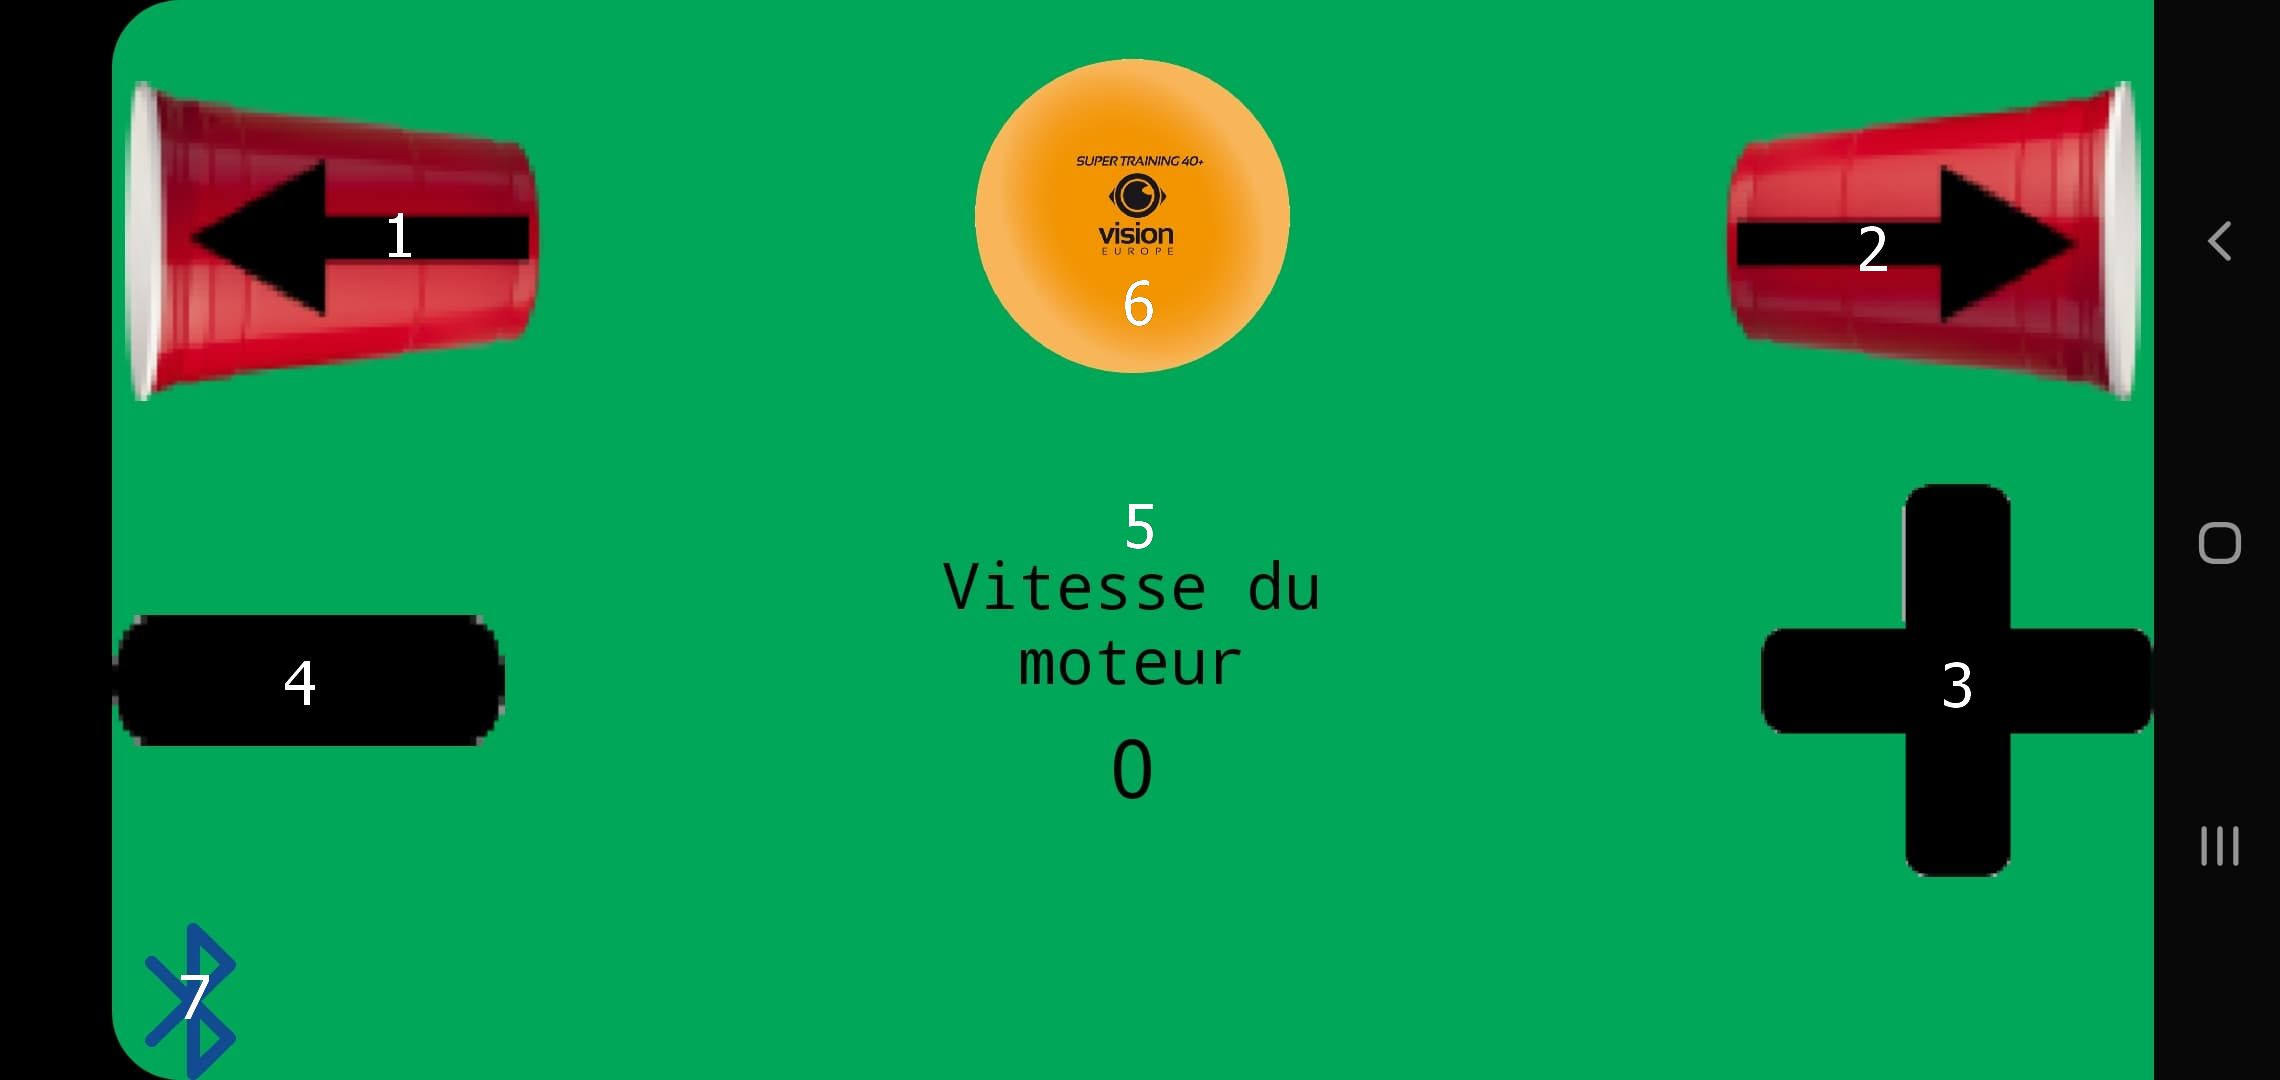
\includegraphics[width=0.6\linewidth]{img/a1/Application}
    \caption{Interface de l'aplication}
    \label{fig:a1-Application}
\end{figure}
